\documentclass[]{beamer}

\mode<presentation>
{
  \usetheme{Warsaw}
  % or ...

  \setbeamercovered{transparent}
  % or whatever (possibly just delete it)
}

\usepackage{xunicode}
\usepackage[slantfont,boldfont]{xeCJK}
\usepackage{ulem}

\setCJKmainfont{AR PL UKai CN}

\XeTeXlinebreaklocale "zh"
\XeTeXlinebreakskip = 0pt plus 1pt


\graphicspath{{./thinking_in_se/}}

\title[Thinking in SE]
{软件工程思想}

\subtitle
{软件工程导论之五} % (optional)

\author[\url{http://sunner.cn}] % (optional, use only with lots of authors)
{王宇颖 \and 孙志岗}
% - Use the \inst{?} command only if the authors have different
%   affiliation.

\institute[哈尔滨工业大学] % (optional, but mostly needed)
{
  计算机科学与技术学院\\
  哈尔滨工业大学}
% - Use the \inst command only if there are several affiliations.
% - Keep it simple, no one is interested in your street address.

\date[Short Occasion] % (optional)
{2011-10-10}

\subject{Slides}
% This is only inserted into the PDF information catalog. Can be left
% out. 



% If you have a file called "university-logo-filename.xxx", where xxx
% is a graphic format that can be processed by latex or pdflatex,
% resp., then you can add a logo as follows:

% \pgfdeclareimage[height=0.5cm]{university-logo}{university-logo-filename}
% \logo{\pgfuseimage{university-logo}}



% Delete this, if you do not want the table of contents to pop up at
% the beginning of each subsection:
\AtBeginSubsection[]
{
  \begin{frame}<beamer>{主要内容}
    \tableofcontents[currentsection,currentsubsection]
  \end{frame}
}


% If you wish to uncover everything in a step-wise fashion, uncomment
% the following command: 

%\beamerdefaultoverlayspecification{<+->}


\begin{document}

\begin{frame}
  \titlepage
\end{frame}

\begin{frame}{主要内容}
  \tableofcontents
  % You might wish to add the option [pausesections]
\end{frame}


% Since this a solution template for a generic talk, very little can
% be said about how it should be structured. However, the talk length
% of between 15min and 45min and the theme suggest that you stick to
% the following rules:  

% - Exactly two or three sections (other than the summary).
% - At *most* three subsections per section.
% - Talk about 30s to 2min per frame. So there should be between about
%   15 and 30 frames, all told.

\section{好的软件}

\subsection[什么是好软件]{什么样的软件是好软件?}

\newenvironment{iconblock}[2]{
    \begin{block}{#1}
    \begin{center}
    \includegraphics[height=2.4cm]{#2}}
{\end{center}
    \end{block}
}

\begin{frame}{下面哪个软件好?}
  \begin{columns}[T]
    \begin{column}{4cm}
      \begin{iconblock}{腾讯QQ}{qq.jpg}\end{iconblock}
      \begin{iconblock}{植物大战僵尸}{pvz.jpg}\end{iconblock}
    \end{column}
    \begin{column}{4cm}
      \begin{iconblock}{Internet Explorer}{ie.png}\end{iconblock}
      \begin{iconblock}{Microsoft Word}{word.png}\end{iconblock}
    \end{column}
  \end{columns}

\end{frame}

\subsection{好软件的特质}

\begin{frame}{用户如何评价软件}
  \begin{description}[正确性]
    \item[正确性] 是否能完成我想要做的事?结果正确吗?
      \pause
    \item[易用性] 学起来容易吗?用起来方便吗?
      \pause
    \item[性能] 速度快不快?吃内存吗?
      \pause
    \item[安全性] 黑客能侵入它吗?后门有木有?
      \pause
    \item[稳定性] 经常死机吗?
      \pause
    \item[成本] 点卡贵不贵?装备怎么卖?
  \end{description}
\end{frame}

\begin{frame}{内行如何评价软件}
  \begin{block}{}
    内行也关注用户所关注的,但还有更多\dots
  \end{block}
  \begin{columns}[t]
    \begin{column}{.5\paperwidth}
      \begin{itemize}
        \pause
        \item 容易修改和扩充吗?\structure{[扩展性]}
          \begin{itemize}
            \item 用户需求总是变化
            \item 竞争的压力山大
          \end{itemize}
        \pause
        \item 代码可多软件共享吗?\structure{[复用性]}
          \begin{itemize}
            \item 降低成本
            \item 代码更可靠
          \end{itemize}
        \pause
        \item 做了充分测试吗?\structure{[可测性]}
        \pause
      \end{itemize}
    \end{column}
    \begin{column}{.5\paperwidth}
      \begin{itemize}
        \item 新人能快速融入吗?\structure{[可维护]}
          \begin{itemize}
            \item 开发人员流动快
            \item 小白经验不足
          \end{itemize}
        \pause
        \item 能在多平台使用吗?\structure{[可移植性]}
          \begin{itemize}
            \pause
            \item Windows, Linux, Mac\dots
            \pause
            \item IE, Firefox, Chrome\dots
            \pause
            \item PC, iPhone, iPad, Android, PSP\dots
          \end{itemize}
        \pause
        \item \dots
      \end{itemize}
    \end{column}
  \end{columns}
\end{frame}

\begin{frame}{好软件的特质}
  \begin{block}{目标}
    \begin{center}
      \Huge 造好的软件!
    \end{center}
  \end{block}
  \pause
  \begin{block}{}
    \begin{center}
      \LARGE 用户和内行都说好,才是真的好
    \end{center}
  \end{block}
  \pause
  \begin{block}{}
    \begin{center}
      \LARGE \alert{矛盾}了怎么办?
    \end{center}
  \end{block}
\end{frame}

\begin{frame}{矛盾}
  \begin{block}{用户和内行的矛盾}
    \begin{center}
      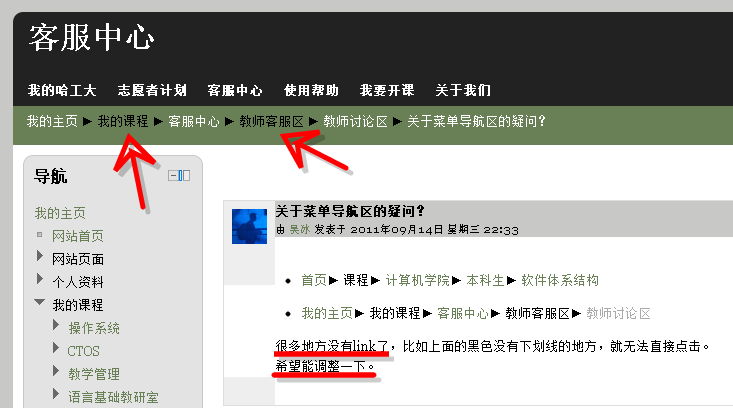
\includegraphics[height=5cm]{cms_navbar.png}
    \end{center}
  \end{block}
\end{frame}

\begin{frame}{矛盾}
  \begin{block}{特质之间的矛盾}
    \begin{columns}
      \begin{column}{.4\textwidth}
        \begin{itemize}
          \item 安全性 vs. 性能
          \item 安全性 vs. 易用性
          \item 可维护 vs. 性能
          \item 可测性 vs. 成本
        \end{itemize}
      \end{column}
      \begin{column}{.6\textwidth}
        
\includegraphics[height=5cm]{contradiction.jpg}
      \end{column}
    \end{columns}
  \end{block}
\end{frame}

\begin{frame}{造好的软件}
  \begin{alertblock}{应对矛盾}
    \begin{center}
      \Huge 折中!
    \end{center}
  \end{alertblock}
  \pause
  \begin{block}{手段}
    \begin{center}
      \Huge 软件生产工程化
    \end{center}
  \end{block}
\end{frame}

\section{软工核心思想}

\subsection{核心之核心}

\begin{frame}{核心之核心}
  \begin{block}{核心思想的核心的核心}
    \begin{center}
      \Huge 向传统工业致敬
    \end{center}
  \end{block}
  \begin{center}
    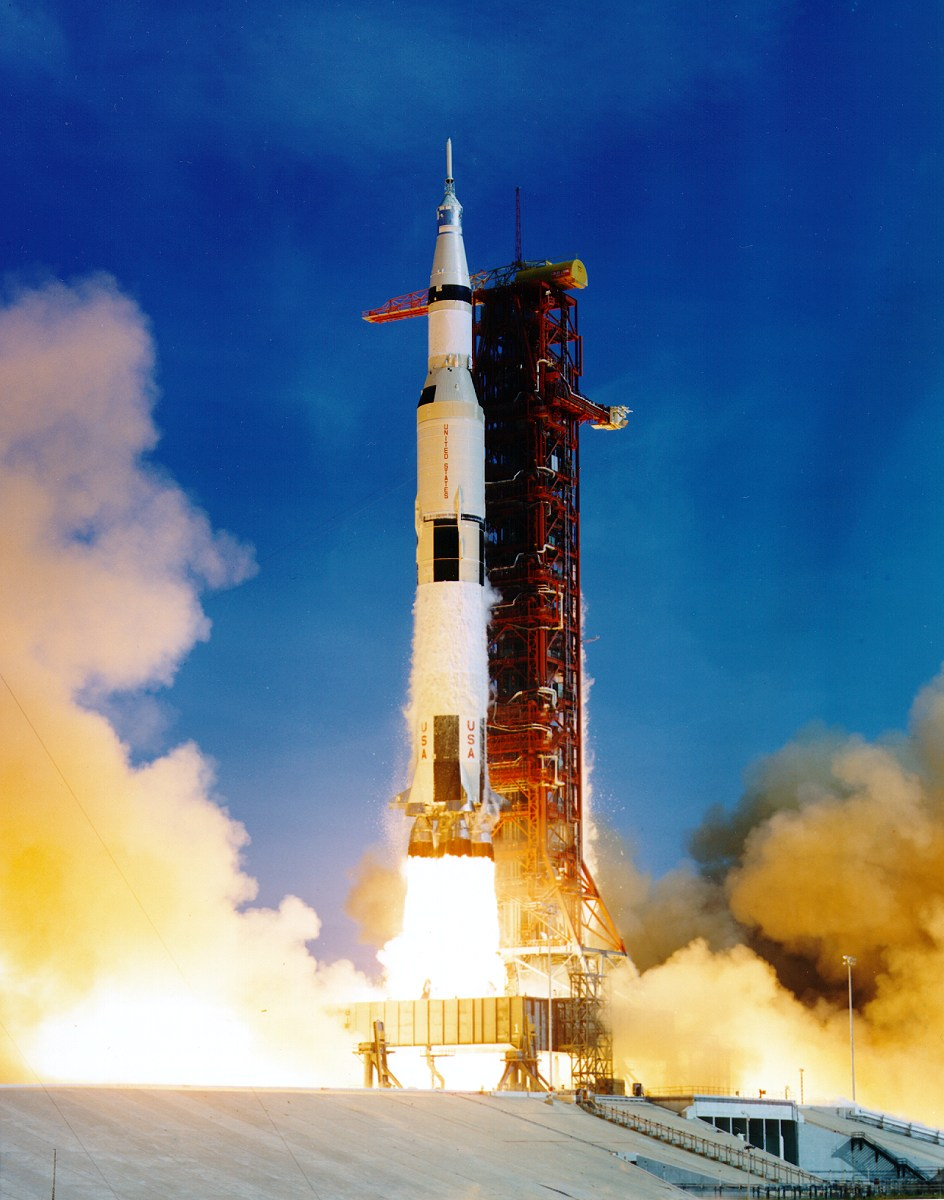
\includegraphics[height=3cm]{spacecraft.jpg}
    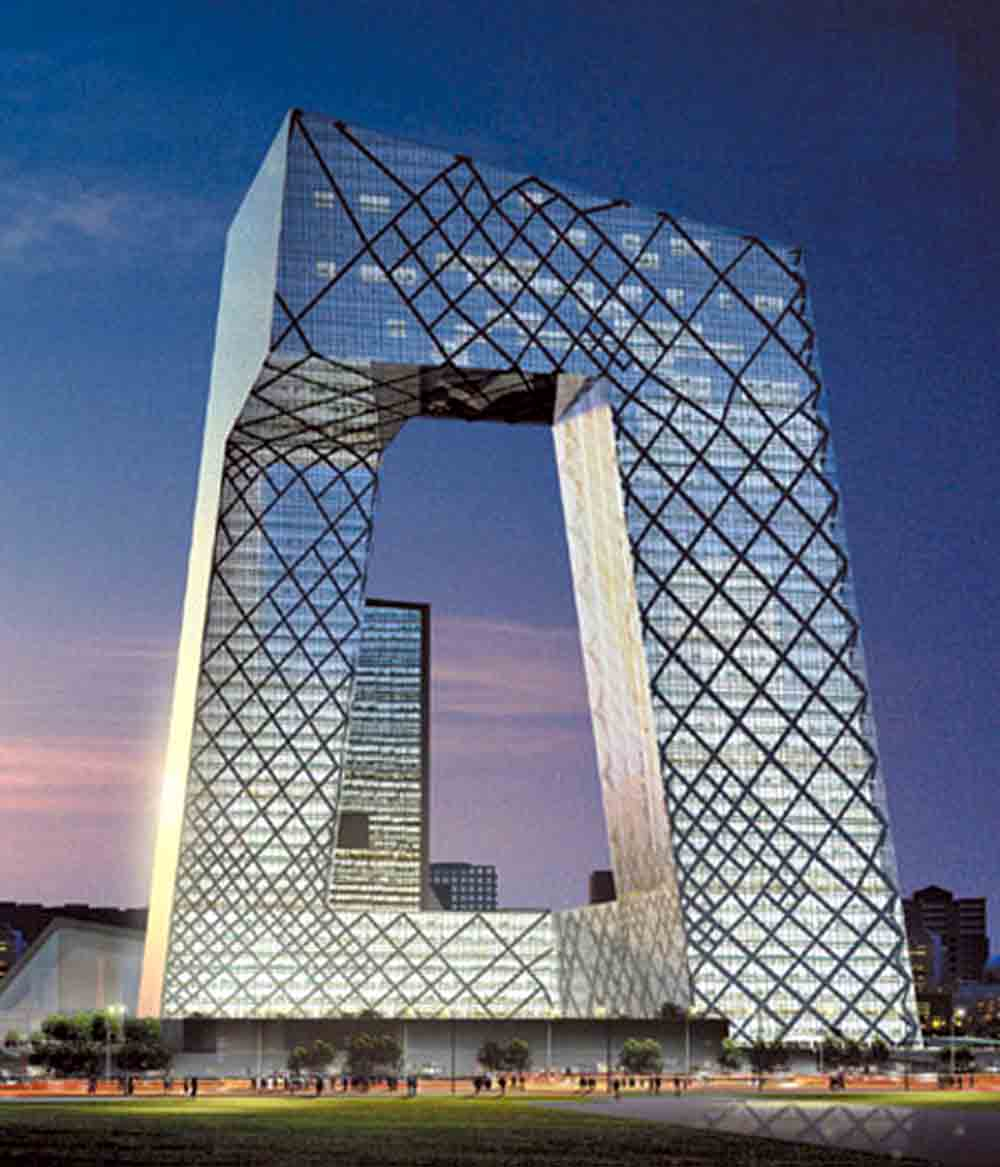
\includegraphics[height=3cm]{cctv.jpg}
    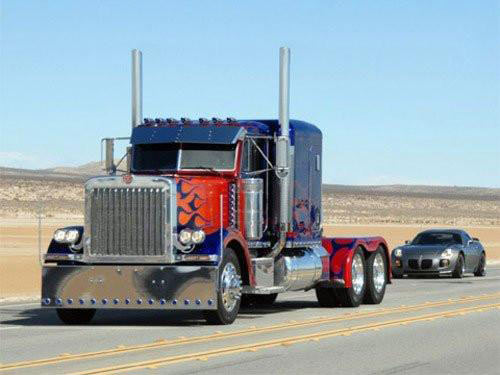
\includegraphics[height=3cm]{prime_trunk.jpg}

    并让传统工业变成\dots
  \end{center}
\end{frame}

\begin{frame}{智能化传统工业}
  \begin{center}
    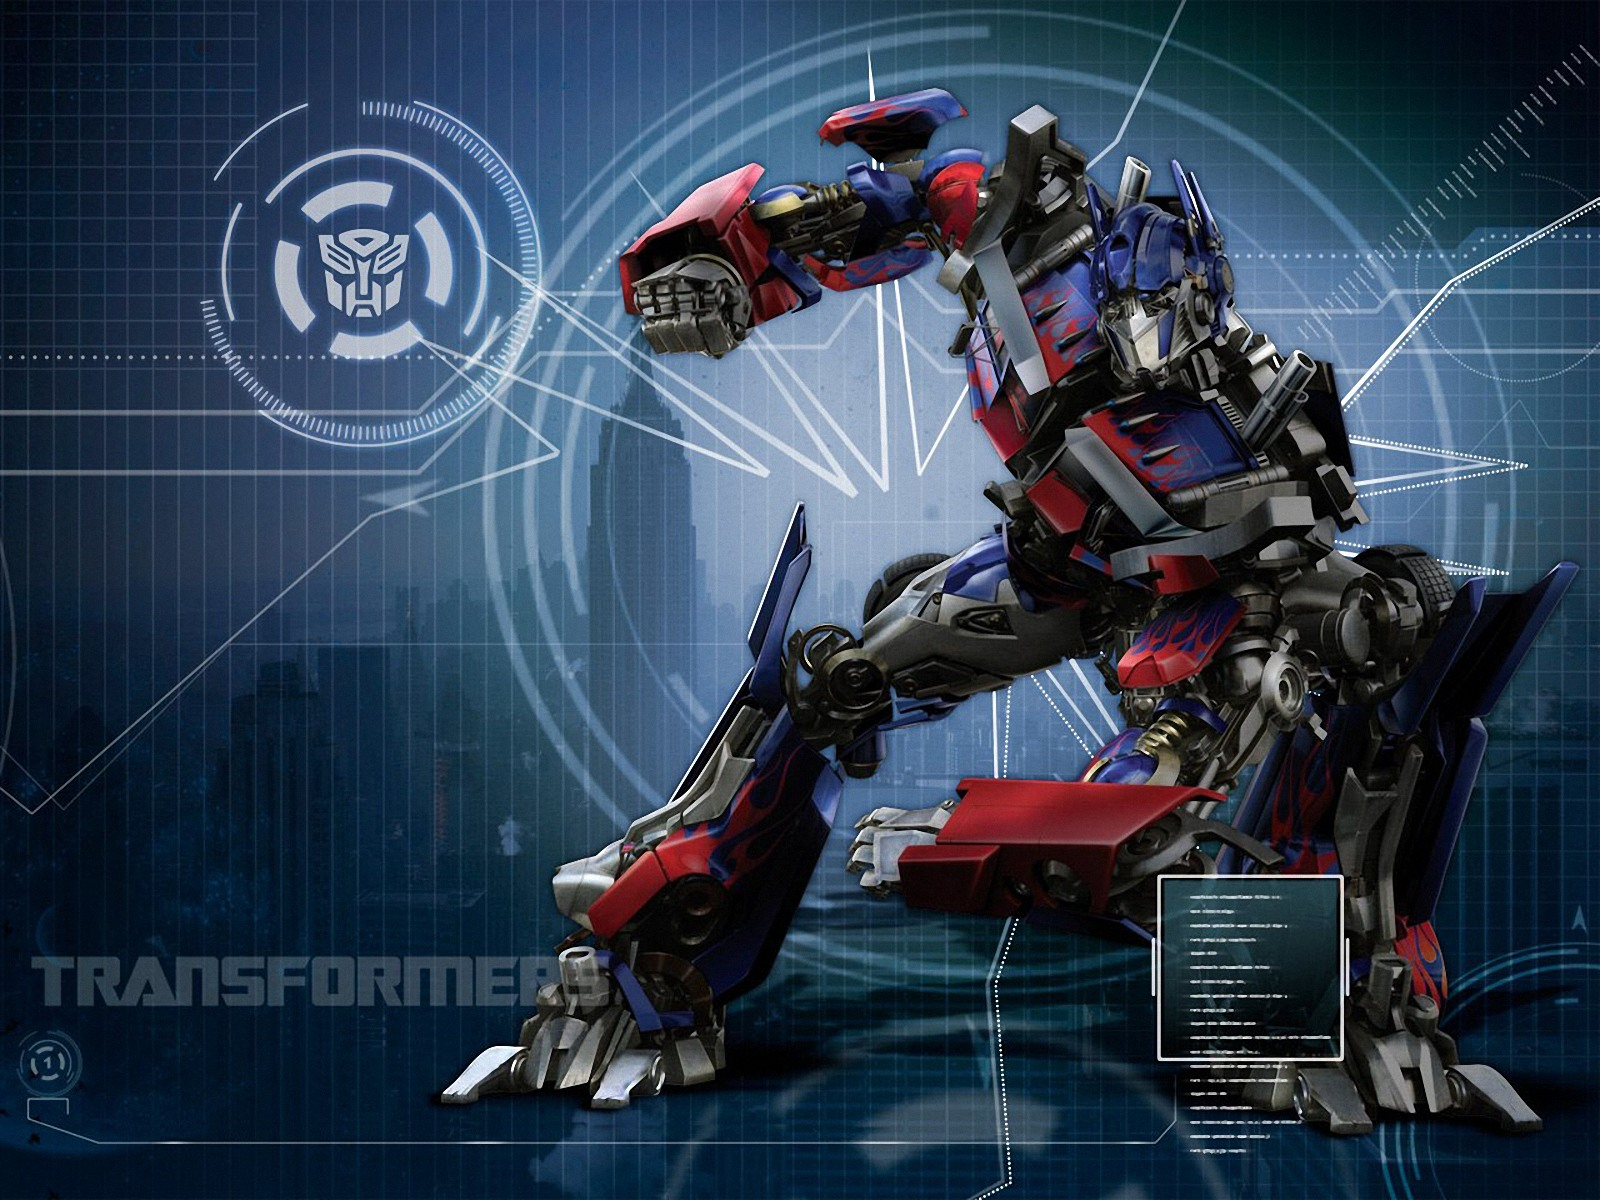
\includegraphics[height=6.5cm]{prime_robot.jpg}
  \end{center}
\end{frame}

\begin{frame}{核心之核心}
  \begin{block}{核心思想的核心的核心}
    \begin{center}
      \alt<1,2>{向传统工业致敬}{向传统工业\alert{\sout{致敬}}挑战}
    \end{center}
  \end{block}
  \begin{block}{核心思想的核心}
    \begin{columns}
      \begin{column}{.3\textwidth}
        \begin{itemize}
          \item 信息隐藏
            \pause
          \item 代码复用
            \pause
          \item 适应变化
        \end{itemize}
      \end{column}
      \begin{column}{.6\textwidth}
        \includegraphics<1>[height=5cm]{car_in_parts.jpg}
        \includegraphics<2>[height=5cm]{screw.jpg}
        \includegraphics<3>[trim=2cm 0cm 0cm 0cm, height=5cm]{chaina.jpg}
      \end{column}
    \end{columns}
  \end{block}
\end{frame}

\subsection{管理}

\begin{frame}{}
  \begin{block}{管理什么?}
    \begin{center}
      \LARGE 管理软件生产过程,及过程中的人
    \end{center}
  \end{block}
  \pause
  \begin{block}{管理思想}
    \begin{columns}
      \begin{column}{.6\textwidth}
        \begin{itemize}
          \item \alert{规格严格}式管理 \--- \structure{[工厂模式]}
            \pause
          \item \alert{功夫到家}式管理 \--- \structure{[敏捷模式]}
        \end{itemize}
      \end{column}
      \begin{column}{.4\textwidth}
        \includegraphics<1,2>[height=3cm]{factory.jpg}
        \includegraphics<3>[height=3cm]{james_bond.jpg}
      \end{column}
    \end{columns}
  \end{block}
\end{frame}

\subsection{技术}

\subsubsection{模块化}

\begin{frame}{模块化}
  \begin{columns}
    \begin{column}{.5\textwidth}
      \begin{block}{}
        1972年,David L. Parnas总结了\structure{信息隐藏},提出软件要\structure{模块化}的思想。
      \end{block}
      \pause
      \begin{block}{从此,软件就不再是个体户了\dots}
        \begin{itemize}
          \item 分层
          \item 分块
          \item 分工
          \item 模块可复用
          \item 重新组合模块以适应变化
        \end{itemize}
      \end{block}
    \end{column}
    \begin{column}{.5\textwidth}
      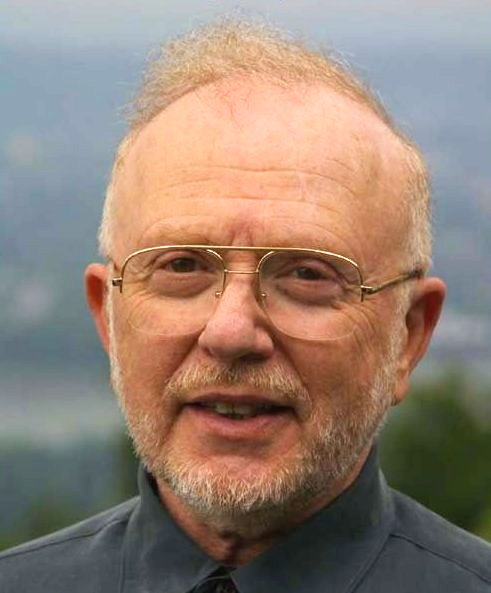
\includegraphics[width=5cm]{parnas.jpg}
    \end{column}
  \end{columns}
\end{frame}

\subsubsection{面向对象}

\begin{frame}{面向对象 (Object-Oriented)}
  \begin{columns}
    \begin{column}{.33\textwidth}
      \begin{block}{2001年图灵奖}
        \begin{center}
          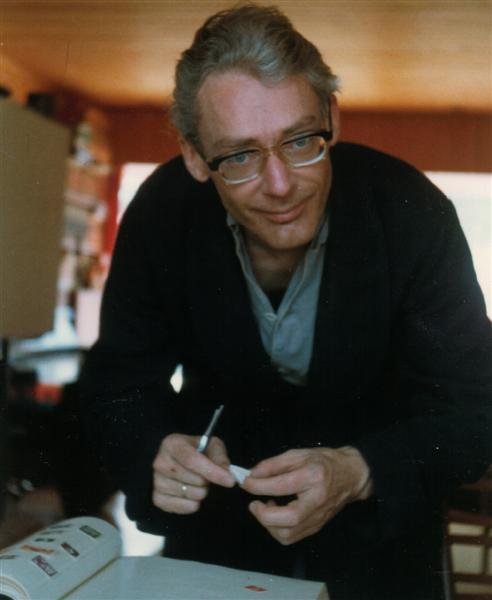
\includegraphics[height=4cm]{dahl.jpg}

          Ole-Johan Dahl
        \end{center}
      \end{block}
    \end{column}
    \begin{column}{.33\textwidth}
      \begin{block}{2001年图灵奖}
        \begin{center}
          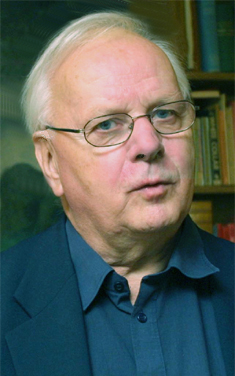
\includegraphics[height=4cm]{kristen.jpg}

          Kristen Nygaard
        \end{center}
      \end{block}
    \end{column}
  \end{columns}
\end{frame}

\begin{frame}{面向对象 (Object-Oriented)}
  \begin{columns}
    \begin{column}{.33\textwidth}
      \begin{block}{2003年图灵奖}
        \begin{center}
          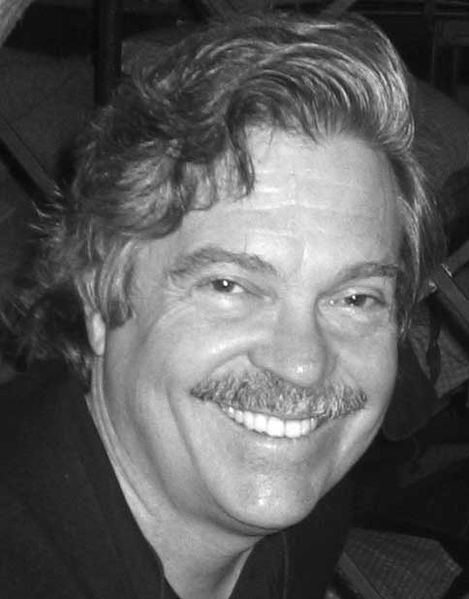
\includegraphics[height=4cm]{kay.jpg}

          Alan Kay
        \end{center}
      \end{block}
    \end{column}
    \begin{column}{.33\textwidth}
      \begin{block}{2008年图灵奖}
        \begin{center}
          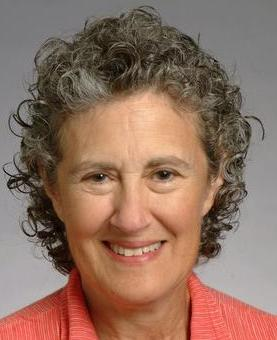
\includegraphics[height=4cm]{liskov.jpg}

          Babara Liskov
        \end{center}
      \end{block}
    \end{column}
  \end{columns}
\end{frame}

\begin{frame}{面向对象}
  \begin{columns}
    \begin{column}{.5\textwidth}
      \begin{itemize}
        \item 一种用计算机程序表示物理世界的哲学
          \pause
        \item 模块化、复用、扩展\dots
          \pause
        \item 指导软件开发的整个过程
        \item \dots
      \end{itemize}
    \end{column}
    \begin{column}{.5\textwidth}
      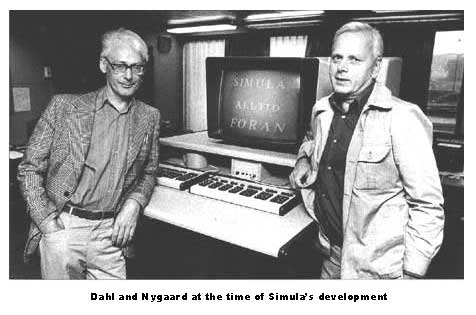
\includegraphics[width=5cm]{dahl_nygaard.jpg}
    \end{column}
  \end{columns}
\end{frame}

\subsubsection{面向构件}

\begin{frame}[fragile]{面向构件}
  \begin{itemize}
    \item 软件间的高层协作
    \item 媒介是通行的接口规范
    \item 无需深入了解彼此
  \end{itemize}
  \pause
  \begin{block}{例如:Unix/Linux的\alert{管道}操作}
    \begin{semiverbatim}
    {\color{magenta}# 列出工大英文主页拼写错误的单词}
    \structure{curl} \alert{"http://en.hit.edu.cn/"} 2>/dev/null {\color{cyan}|}
    \structure{sed} \alert{'s/[^a-zA-Z ]/ /g'} {\color{cyan}|}
    \structure{tr} \alert{'A-Z ' 'a-z\\n'} {\color{cyan}|}
    \structure{grep} \alert{'[a-z]'} {\color{cyan}|}
    \structure{sort} -u {\color{cyan}|}
    \structure{comm} -23 - <(\structure{sort} /usr/share/dict/words) {\color{cyan}|}
    \structure{less}
    \end{semiverbatim}
  \end{block}
\end{frame}

\begin{frame}{面向构件---微软的COM技术}
  \begin{columns}
    \begin{column}{0.4\textwidth}
      \begin{block}{}
        腾讯QQ浏览器 \tikz[na] \coordinate (s-qq);
      \end{block}
    \end{column}
    \begin{column}{0.4\textwidth}
      \begin{block}{}
        微软Internet Explorer \tikz[na] \coordinate (s-ie);
      \end{block}
    \end{column}
  \end{columns}
  \begin{center}
    % Use a background grid to make it easier to find coordinates
    % When the coordinates have been found, remove the 
    % 'show background grid' option. 
    \tikzstyle{background grid}=[draw, black!50,step=.5cm]
    \begin{tikzpicture}%[show background grid]
      % Put the graphic inside a node. This makes it easy to place the
      % graphic and to draw on top of it. 
      % The above right option is used to place the lower left corner
      % of the image at the (0,0) coordinate. 
      \node [inner sep=0pt,above right] 
      {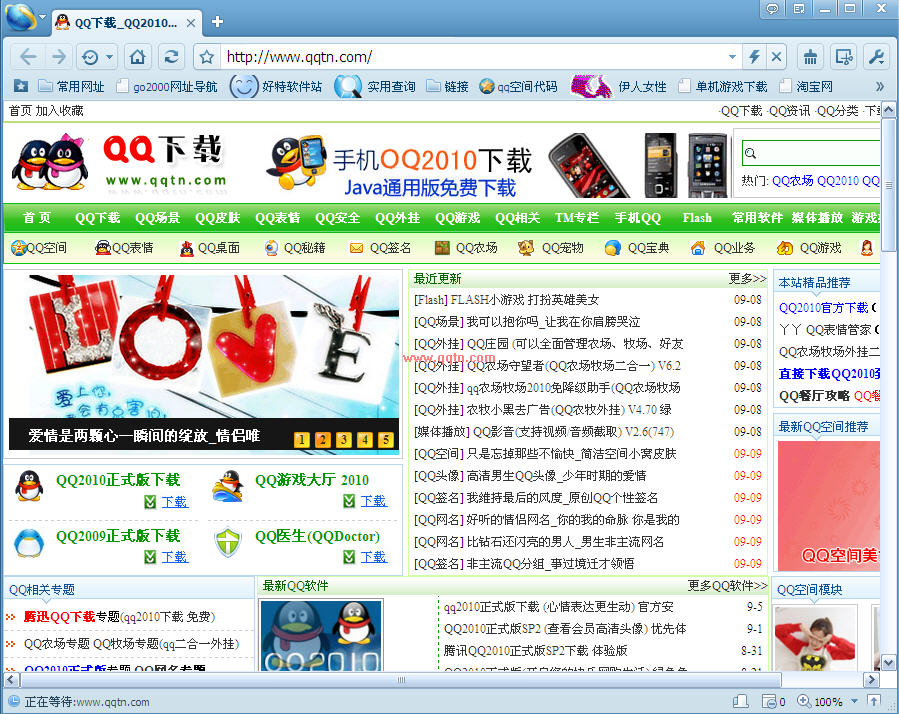
\includegraphics[width=10cm]{qqbrowser.jpg}};
      % define destination coordinates
      \path (4.5, 7.3) coordinate (qq)
            (5, 4.5) coordinate (ie)
            (0, 6.85) coordinate (qqzone1)
            (10, 8) coordinate (qqzone2)
            (0, 1) coordinate (iezone1)
            (9.8, 6.8) coordinate (iezone2);
    \end{tikzpicture}
  \end{center}

  % define overlays
  % Note the use of the overlay option. This is required when 
  % you want to access nodes in different pictures.
  \only<2->{
    \begin{tikzpicture}[overlay]
      \path[->,red,ultra thick] (s-qq) edge [bend right] (qq);
      \draw [dashed, red, ultra thick] (qqzone1) rectangle (qqzone2);
    \end{tikzpicture}
  }
  \only<3>{
    \begin{tikzpicture}[overlay]
      \path[->,blue,ultra thick] (s-ie) edge [bend left] (ie);
      \draw [dashed, blue, ultra thick] (iezone1) rectangle (iezone2);
    \end{tikzpicture}
  }
\end{frame}

\begin{frame}{面向构件---Web上的Mashup}
  \begin{columns}
    \begin{column}{0.4\textwidth}
      \begin{block}{}
        京东网上商城 \tikz[na] \coordinate (s-360buy);
      \end{block}
    \end{column}
    \begin{column}{0.4\textwidth}
      \begin{block}{}
        百度地图 \tikz[na] \coordinate (s-baidu);
      \end{block}
    \end{column}
  \end{columns}
  \begin{center}
    % Use a background grid to make it easier to find coordinates
    % When the coordinates have been found, remove the 
    % 'show background grid' option. 
    \tikzstyle{background grid}=[draw, black!50,step=.5cm]
    \begin{tikzpicture}%[show background grid]
      % Put the graphic inside a node. This makes it easy to place the
      % graphic and to draw on top of it. 
      % The above right option is used to place the lower left corner
      % of the image at the (0,0) coordinate. 
      \node [inner sep=0pt, above right] 
      {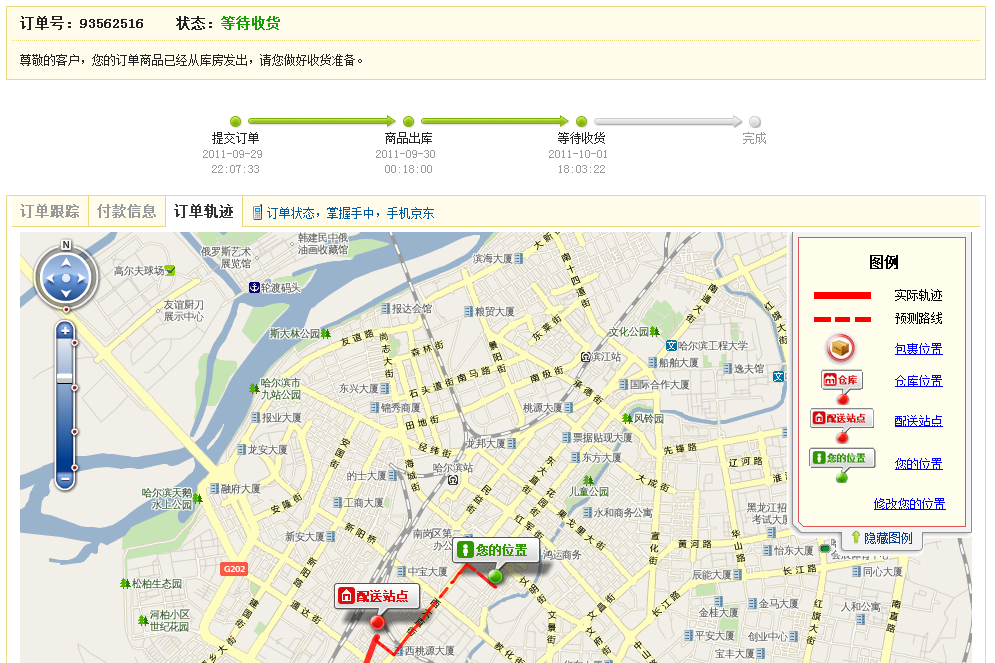
\includegraphics[width=10cm]{360buy.png}};
      % define destination coordinates
      \path (4.5, 5.5) coordinate (360buy)
            (5, 3) coordinate (baidu)
            (0, 4.35) coordinate (3zone1)
            (10, 6.6) coordinate (3zone2)
            (0.25, 0.5) coordinate (bzone1)
            (9.75, 4.3) coordinate (bzone2);
    \end{tikzpicture}
  \end{center}

  % define overlays
  % Note the use of the overlay option. This is required when 
  % you want to access nodes in different pictures.
  \only<2->{
    \begin{tikzpicture}[overlay]
      \path[->,red,ultra thick] (s-360buy) edge [bend right] (360buy);
      \draw [dashed, red, ultra thick] (3zone1) rectangle (3zone2);
    \end{tikzpicture}
  }
  \only<3>{
    \begin{tikzpicture}[overlay]
      \path[->,blue,ultra thick] (s-baidu) edge [bend left] (baidu);
      \draw [dashed, blue, ultra thick] (bzone1) rectangle (bzone2);
    \end{tikzpicture}
  }
\end{frame}

\subsubsection{中间件}
\begin{frame}{中间件}
  \begin{alertblock}{问题}
    构件繁多,各说各话
  \end{alertblock}
  \pause
  \begin{block}{中间件}
    \begin{itemize}
      \item 做方言与普通话的翻译
      \item 使用普通话的构件,便可以与方言沟通
    \end{itemize}
  \end{block}
  \pause
  \begin{block}{例如}
    \begin{itemize}
      \item 短信网关使不同运营商间的短信互通
      \item 支付宝协调各种支付方式
    \end{itemize}
  \end{block}
\end{frame}

\begin{frame}{回顾}
  \begin{columns}
    \begin{column}{0.5\textwidth}
      \tableofcontents[pausesections]
    \end{column}
    \pause
    \begin{column}<3->{0.5\textwidth}
      \begin{block}{}
        \begin{center}
        \large 这都是笼统的\structure{凤毛麟角}\dots

        \huge \alert{欢迎提问,

        谢谢!}
        \end{center}
      \end{block}
    \end{column}
  \end{columns}
\end{frame}

\end{document}
